% What is still missing in between sections? The pathloss model

\section{Reliability of the IPA algorithm in terms of location probability}\label{sec:contri1}

To determine the maximum transmission power of a secondary transmitter and ensure protection of the primary users, knowledge of the path propagation characteristics is needed. Examples of these characteristics are: the distances between the secondary transmitter and any primary transmitters, terrain shape and the relative antenna discrimination. The latter two characteristics determine the path loss $PL$. Although the characteristics are not known directly by the secondary transmitter, they can be estimated with the IPA algorithm. The distances between the secondary and primary transmitters can be computed with the distance-to-contour flooding algorithm and a local estimation of the path loss is computed with a MLS algorithm. In this section we investigate the reliability of the estimation of the path propagation characteristics by looking at the location probability.

\subsection[title]{Location probability$^2$}

\setcounter{footnote}{2}
\footnotetext{In this section we follow the description given in ECC report 159 \cite{ecc}.}

The location probability $q$ is defined as the probability with which a primary DTT receiver would operate correctly at a specific location, or gridpoint; i.e., the probability with which the median wanted signal level $P_P$ is appropriately greater then a minimum required value ;i.e.,
\begin{equation} \label{eq:lp}
q=Pr\{P_P\geq P_{P,min}+\sum_{i=1}^K r_{S,i}P_{S,i}\}=Pr\{P_P\geq S\} 
\end{equation}
In this formula, $P_{P,min}$ is the primary receiver's (noise-limited) reference sensitivity level \footnote{The reference sensitivity level of a receiver is the minimum wanted signal power for which the receiver can operate correctly in a noise-limited environment.}, $P_{S,i}$ is the received power of the $i^{th}$ unwanted, secondary, DTT signal and $r_{S,i}$ is the DTT-to-DTT protection ratio for the $i^{th}$ DTT transmitter; i.e., the minimum ratio of the wanted signal power and the interference signal power necessary for correct operation of the receiver. In the path loss model used in the simulations, the RSS at a gridpoint is a Gaussian variable were the mean $m$ is determined by the distance from the transmitter, antenna losses and shadowing. The variance $\sigma^2$ is determined by the amount of fast fading. Consider a gridpoint were a receiver senses the primary and secondary transmitter. We compute $Pr\{P_P\geq S\}$ at this gridpoint with Eq.~\ref{eq:lpCDF}.  as illustrated in Fig.~\ref{fig:compLP}. 


% Deze figuur zeker nog aanpassen!!! Letters kloppen niet en kwaliteit is niet ok!
\begin{figure}
\centering
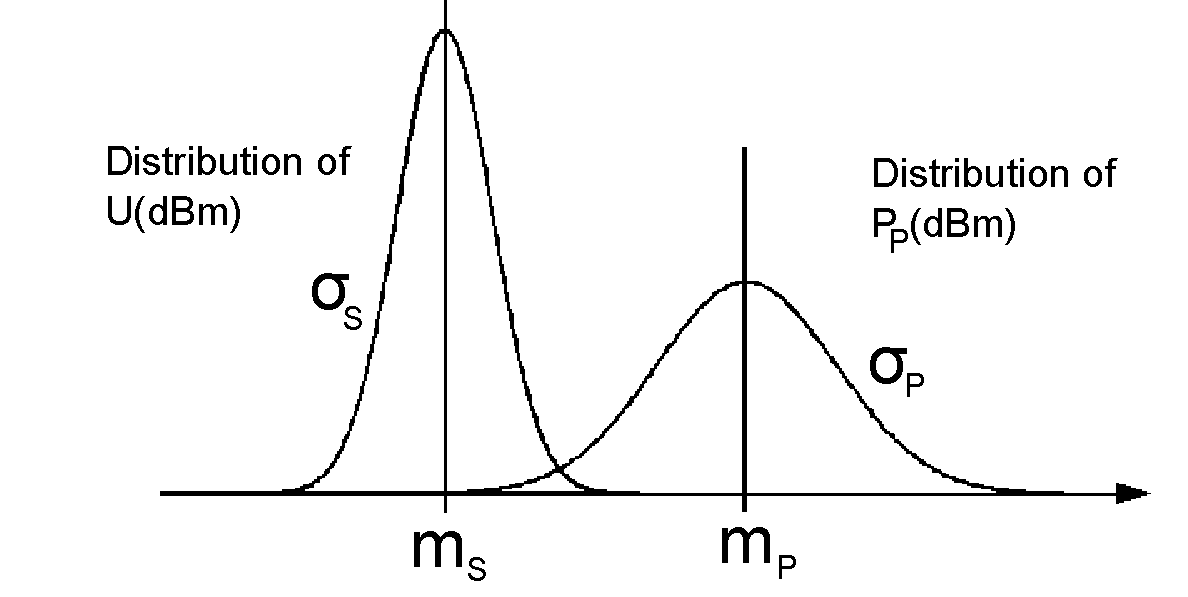
\includegraphics[scale=0.4]{figures/contribution1/distri.pdf}
\caption{\label{fig:compLP} \cite{ecc} The Gaussian distributions of the power of a secondary transmitter $S$ and a primary transmitter $P$ at one gridpoint. To compute the location probability at a location, we compute $Pr\{P_P\geq S\}$.}
\end{figure}

\begin{equation} \label{eq:lpCDF}
q=1-\frac{1}{2}\text{erfc}\{\frac{1}{\sqrt{2}}\frac{m_{S(dBm)}-m_{U(dBm)}}{\sqrt{\sigma_S^2+\sigma_U^2}}\}\
\end{equation}

\subsection{Simulation results}

A simulation of the IPA algorithm is shown in Fig.~\ref{fig:iterationsLP}. The effect of the secondary transmitter on the location probability of the primary transmitter for this simulation is illustrated by the results for example 2 in Tab.~\ref{tab:locProbEffect}. The table also shows the results for two other simulations.

\begin{table}
\caption{\label{tab:locProbEffect}Reliability of the IPA algorithm in terms of the location probability and overlap of the interference threshold contours for three different scenarios. }

\vspace{0mm}
\begin{tabular}{cccc}
\hline
          	&                 & $\Delta$ &	contour				\\
          	&                 & ($\%$)	& overlap ($\%$) PU	\\\hline
 example 1	& update 1				&	7				&	0							\\
 (2000 nodes)&update 2      	&	7				&	0							\\
            & update 3       	&	7.1			& 0							\\\hline 
 example 2	& update 1      	&	8				& 0							\\ 
 (1500 nodes)& update 2				& 9.1			& 0.3						\\\hline
            & update 1 				& 7.9			&	0							\\	
 example 2	& update 2 				& 7.9			&	0							\\	
 (1800 nodes)& update 3 			& 7.9			&	0							\\	
	          & update 4 				& 10.6			&	0							\\\hline		            

\end{tabular}
\vspace{-5mm}
\end{table}

\begin{figure}
\centering
\subfloat[primary transmitter]{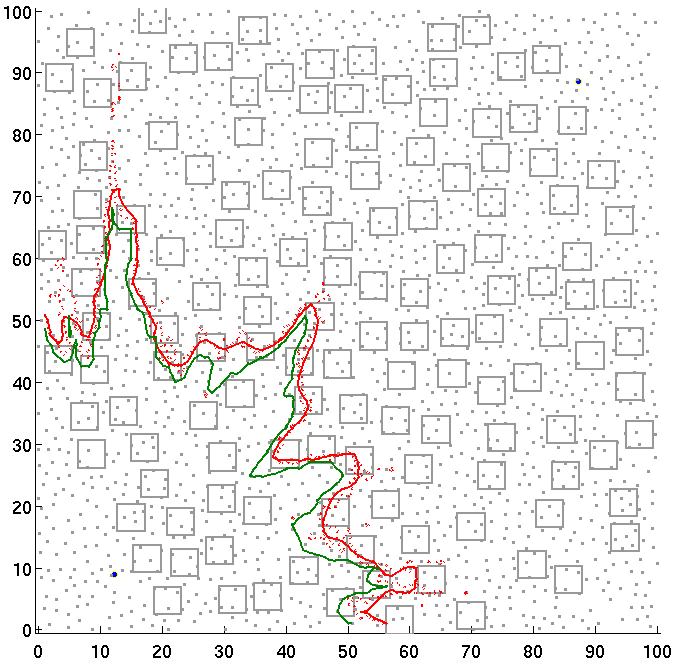
\includegraphics[scale=0.18]{figures/contribution1/vb2it0}} 
\subfloat[update 1]{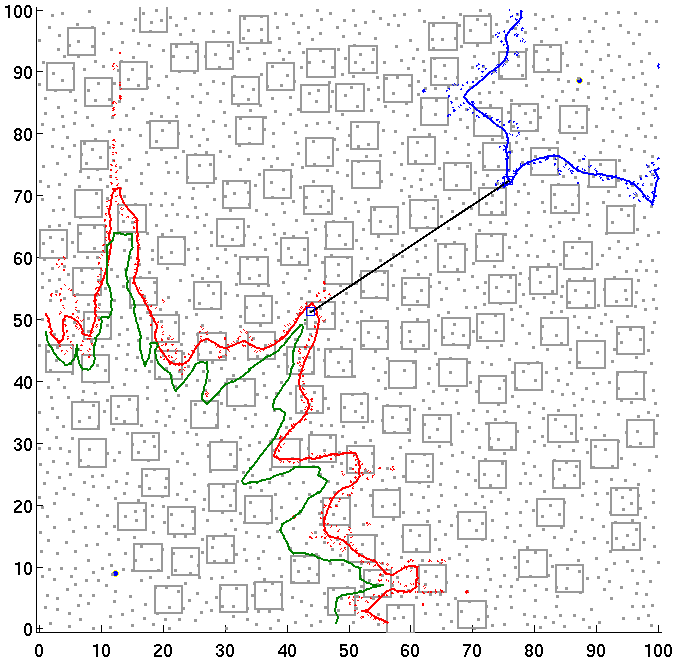
\includegraphics[scale=0.18]{figures/contribution1/vb2it1}} \\
\subfloat[update 2]{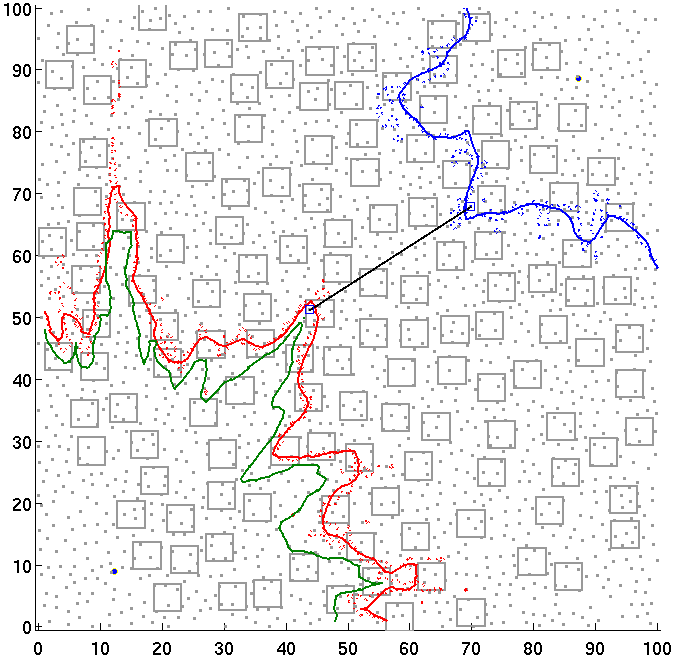
\includegraphics[scale=0.18]{figures/contribution1/vb2it2}}
\subfloat[update 3]{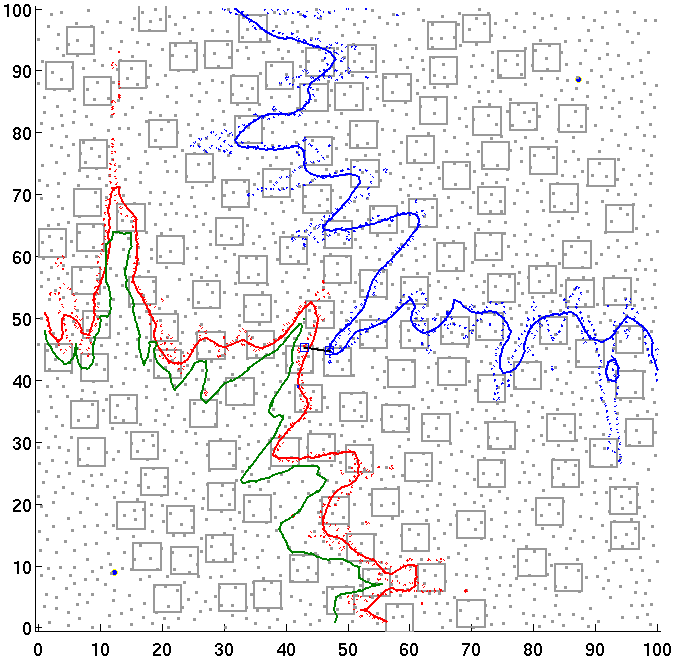
\includegraphics[scale=0.18]{figures/contribution1/vb2it3}}
\caption{\label{fig:iterationsLP} Demonstration of the IPA algorithm for example 2 from 
Tab.~\ref{tab:locProbEffect}. A primary transmitter is present in the lower left corner of the scenario and its interference threshold contour is indicated in red. The $95\%$ location probability contour is indicated in green. In the upper right corner a secondary transmitter is present with the interference contour indicated in blue.}
\end{figure}

In the second column of the table, $\Delta$ indicates the decrease of the area, $A$(textit{with SU}), of the $95\%$ location probability contour of the primary transmitter in comparison with the area of the contour when there is no interference from a secondary transmitter, $A$(\textit{no SU}), as shown in Eq.~\ref{eq:deltalp}. The decrease is indicated for every iteration of the IPA algorithm.

\begin{equation} \label{eq:deltalp}
\Delta=\frac{A(\textrm{\textit{no SU}})-A(\textrm{\textit{with SU}})}{A(\textrm{\textit{no SU}})}
\end{equation}

The third column shows the overlap of the interference threshold contours of the primary and the secondary transmitter as computed by the IPA algorithm. The overlap is expressed as the percentage of the area of the primary transmitter's contour that is overlapped by the contour of the secondary transmitter.

The simulations from Tab.~\ref{tab:locProbEffect} show that the presence of a secondary transmitter reduces the location probability with 7 to 10$\%$. The biggest reduction of the location probability is caused by the presence of a secondary transmitter and not by the increase in power as computed by the IPA algorithm. The reliability of the IPA algorithm is confirmed by Fig.~\ref{fig:connectionLPOverlap}. This figure shows that there is a relationship between the interference threshold contours computed by the IPA algorithm and the location probability. This justifies the use of the propagation contour-contour distance computed by the IPA algorithm as a metric for interference.

\begin{figure}
\centering
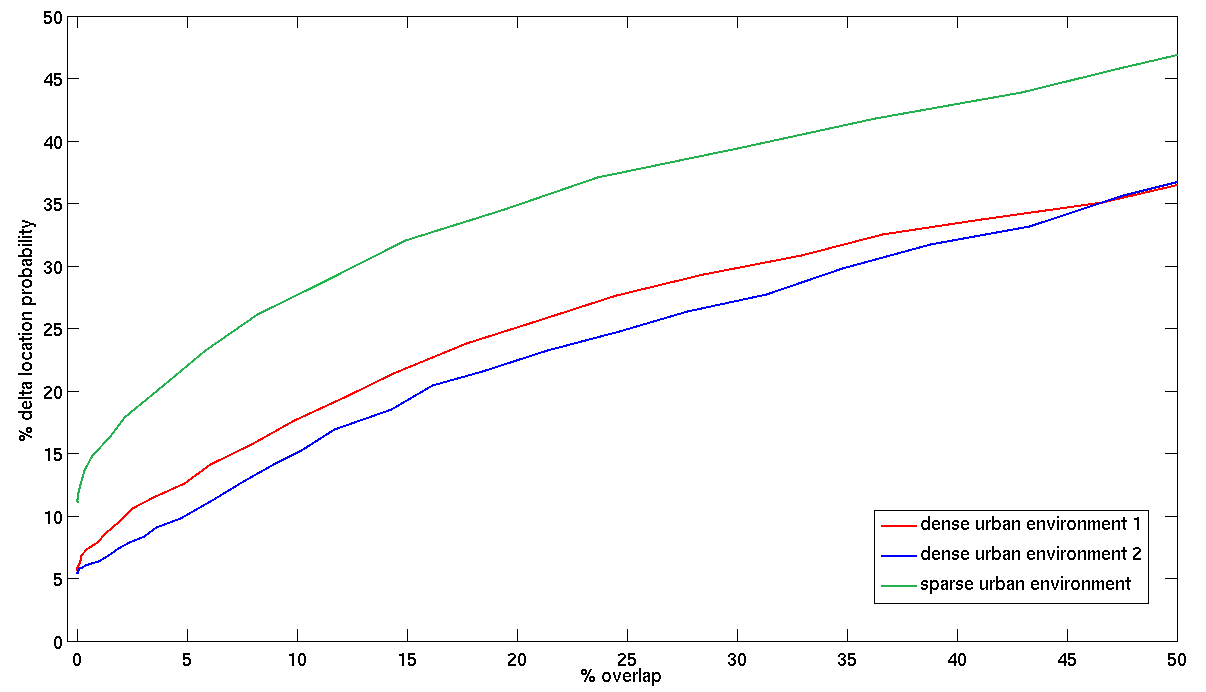
\includegraphics[scale=0.3]{figures/contribution1/correlation.png}
\caption{\label{fig:connectionLPOverlap} Reduction of the $95\%$ location probability contour in function of the overlap of the primary and secondary contour computed by the IPA algorithm.}
\end{figure}

% Remove table 2 since this tells the same story as the figure with the linear connection, it is a snapshot.
% \begin{table}
\caption{Performance of the algorithm for the examples of Fig.~\ref{fig:overlap}.
% the number
%of updates and the percentage of nodes misclassified for each contour propagation.
%Note that the number of updates to propagate the contour 
%is very close to $N$.
}
\vspace{0mm}
\begin{tabular}{ccc}
\hline
          	& 95$\%$ LP &	contour				\\
          	& $\Delta$	& overlap $\%$	\\\hline
 example 1	&	94.49			&	0							\\\hline 
 example 2	&	79.8			& 17.32					\\\hline        

\end{tabular}
\label{tab:overlap}\vspace{-5mm}
\end{table}


\begin{figure}
\centering
\subfloat[]{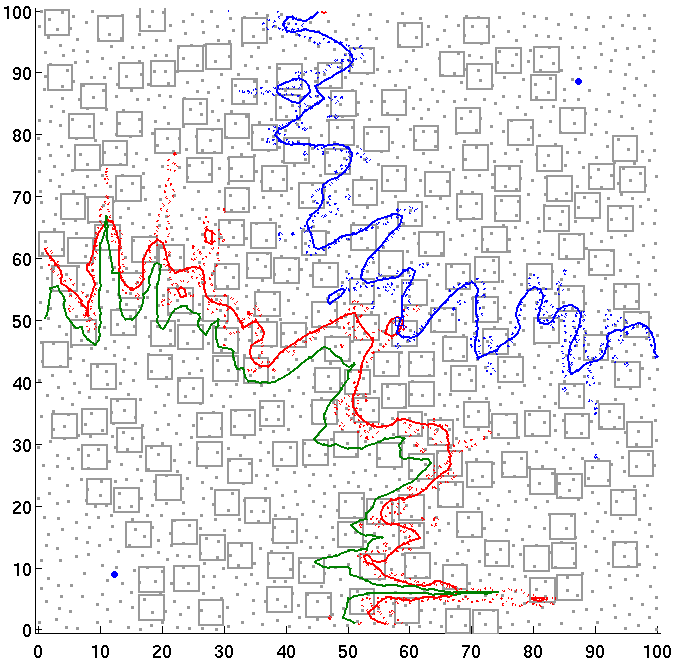
\includegraphics[scale=0.18]{figures/contribution1/vbNoOverlap}} 
\subfloat[]{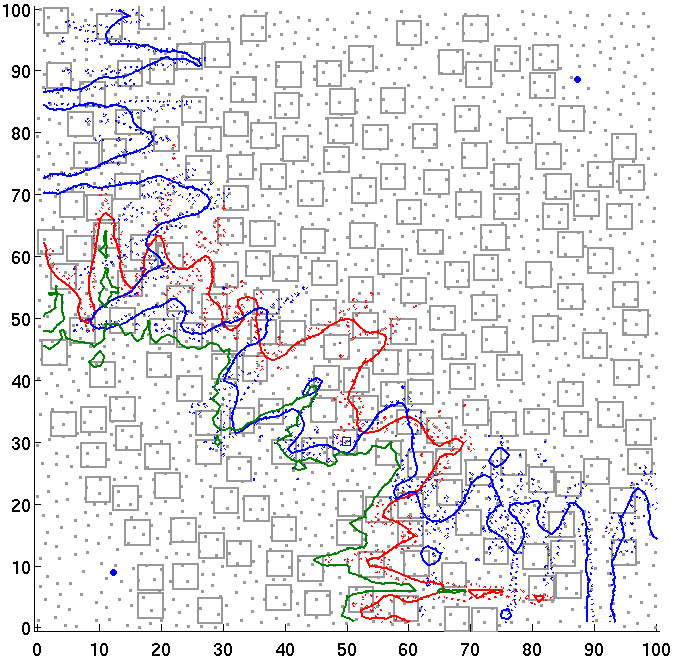
\includegraphics[scale=0.18]{figures/contribution1/vbOverlap}}
\caption{\label{fig:overlap} Demonstration of the effect of the overlap of the contours on the location probability. The results for this scenario are given in Tab.~\ref{tab:overlap} in terms of reduction of the location probability.}
\end{figure}

